\documentclass[a4paper]{article}
\usepackage[T1]{fontenc}
\usepackage[utf8]{inputenc}
\usepackage{lmodern}
\usepackage{graphicx}
\usepackage[left=2.5cm,right=2.5cm,top=3cm,bottom=3cm]{geometry}
\usepackage{eurosym}
\usepackage{fancyhdr}%encabezado y pie de página
\usepackage[colorlinks=true, linkcolor=black, urlcolor=blue]{hyperref}
\setcounter{secnumdepth}{5}
\usepackage[spanish]{babel}
\setcounter{tocdepth}{5}
\usepackage{colortbl}%para colorear tablas
\usepackage{tabularx}
\usepackage{placeins}%para poner barrera y no pasen de secciones los elementos flotantes
%\usepackage{wasysym} %para poner símbolos
\usepackage{bbding} %para poner símbolos



%para el mapa mental
\usepackage{tikz}
\usetikzlibrary{mindmap,trees}
\usepackage{verbatim}


\date{}
\author{D. Ramirez Ambrosi \\ J. I. Sánchez Méndez \\ J. Rodríguez Azpeleta}
\title{\begin{center}
\textbf{\Huge{Make Yourself Strong}} \\ Storyboard  \\Proyecto de la asignatura Interacción Persona Computador \\ \Huge{Grupo 10}
\end{center}}
\date{\today}


\pagestyle{fancy}
\rhead{
\textbf{Make Yourself Strong} \hfill \textbf{Fecha:} \date{\today}
}

\lhead{}

%Separación entre párrafos
\setlength{\parskip}{3mm}

%colores
\definecolor{verde}{RGB}{127,255,0}%color para la barra de titulo
\definecolor{rojo}{RGB}{255,0,0}%color para características
\renewcommand\listfigurename{\centering LISTA DE FIGURAS}

\begin{document}
\maketitle

\thispagestyle{empty}%para evitar enumeración de la página de la portada y del índice
\newpage
\tableofcontents%índice
\thispagestyle{empty}
\newpage



%lista de figuras 
%\renewcommand\listfigurename{\centering LISTA DE FIGURAS}
%\listoffigures
%\clearpage

%Lista de tablas
%\renewcommand{\listtablename}{\centering ÍNDICE DE TABLAS} %Para cambiar el índice de las tablas
%\listoftables
%\thispagestyle{empty}
%\newpage

\setcounter{page}{1}%Para reiniciar el contador de páginas en la página deseada


\section{Inspiraciones}

A continuación exponemos las inspiraciones identificadas para la creación de la aplicación:

\begin{itemize}
	
	\item   \textbf{Tablas de entrenamientos}: Nos sirven de inspiración para la creación de iconos en la página. También para ejemplificar los diferentes ejercicios y mostrar de forma resumida como se deben realizar. La figura \ref{fig:ejemplo} muestra una tabla de entrenamiento.
	
	\item   \textbf{Cuadernos}: Sirven para apuntar cualquier cosa. En ellos se inspirarán los registros de actividad del usuario, tanto la entrada de información como su presentación.
	
	\item   \textbf{Combinación de colores azules, blancos y grises}: Una mezcla de colores que inspire paz y tranquilidad, de forma que los usuarios de la aplicación se sientan cómodos al navegar por la página.
	
	\item  \textbf{\url{ingdirect.es}}: Nos gusta su estilo, su estructuración de menús, su diseño moderno y limpio. Tomaremos ideas de ella para el diseño final de la aplicación.
	
	\item   \textbf{MyFitnessPAL}: Aplicación que hemos encontrado similar a nuestra aplicación objetivo. Esta aplicación se centra principalmente en la nutrición, mientras que nuestro caso la atención principal está en los entrenamientos.
\end{itemize}

\begin{figure}[hbpt]

	\centering
	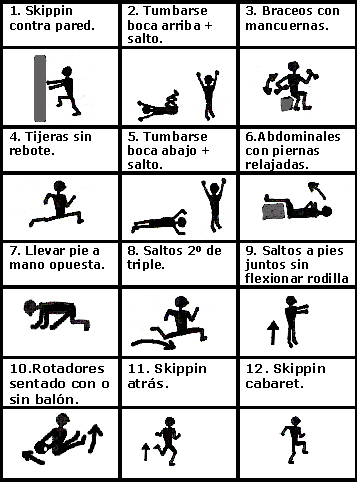
\includegraphics[width=0.7\textwidth]{./figuras/tabla_entr.jpg}
	\caption{Tabla de entrenamiento, en este caso representa una rutina de ejercicios}
	\label{fig:ejemplo}

\end{figure}

\section{Punto de vista}

El punto de vista a desarrollar invita al usuario a darse cuenta de que `\textit{`con buenos consejos, cualquiera puede ser su propio entrenador personal}'' y que ``\textit{ponerse en forma es fácil con un poco de ayuda}''. De esta forma, no hace falta contratar los servicios de un entrenador personal o apuntarse a un grupo organizado con horarios rigurosos e inflexibles. En cierta forma permite ``\textit{disponer de flexibilidad de horarios}'' y ``\textit{otorga la capacidad de organizar los entrenamientos propios sin dependencias de horarios o personas}''.

Evidentemente, estos últimos puntos no son tan flexibles como uno quisiera desear. Como en cualquier otro campo, alcanzar una meta requiere dedicación y esfuerzo, para lo que se requiere regularidad. Sin embargo, el hecho de no tener que depender de estar a una hora concreta en cierto sitio o esperar que alguien asigne los ejercicios a realizar sí que permite una mayor flexibilidad al usuario, que puede ser autosuficiente.

También cabe mencionar el cambio en el tema de la página que hemos visto necesario. Inicialmente, el foco de atención se centraba en el \textbf{entrenamiento de fuerza} y, actualmente, el tema ha sido abierto y ampliado al \textbf{entrenamiento físico en general}, llegando a incluir en segundo plano el tema de la \textbf{alimentación} y nutrición.

\FloatBarrier
\section{Storyboard}

\begin{figure}[!h]
\centering
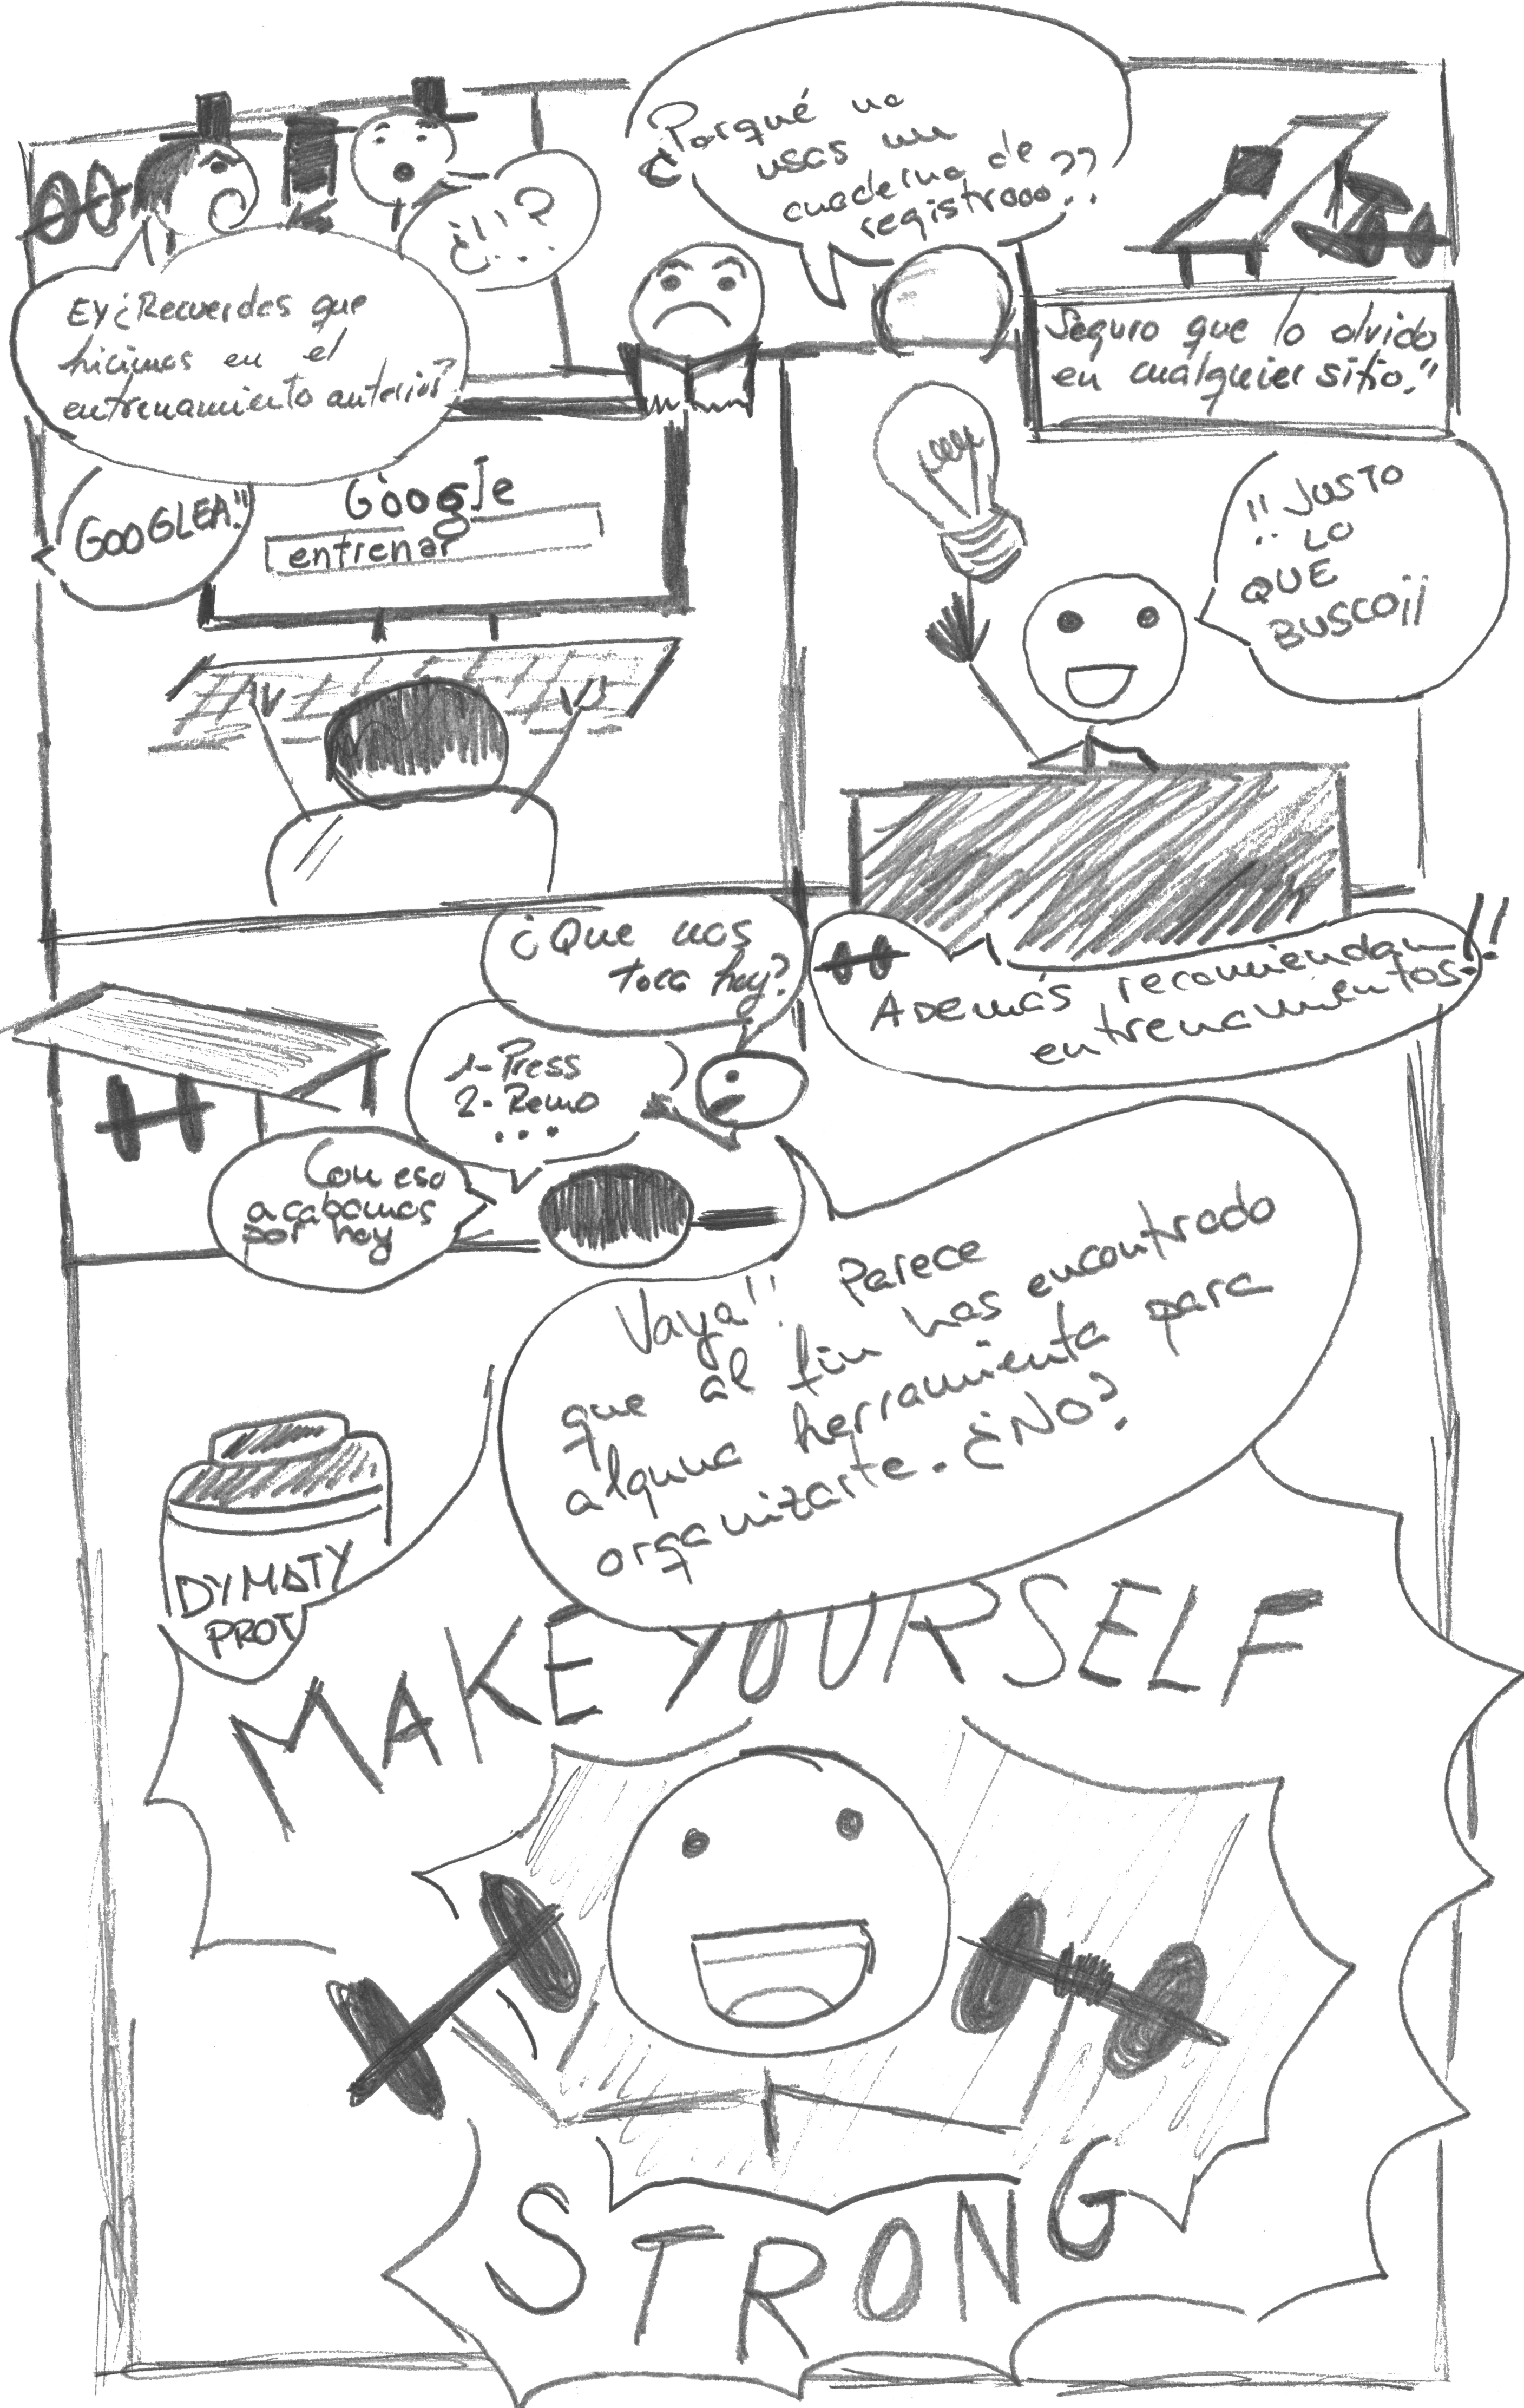
\includegraphics[width=0.85\textwidth]{./figuras/storyboard1-mas-negro.jpg}
\caption{Story board 1}
\end{figure}

\begin{figure}[!h]
\centering
\includegraphics[width=0.95\textwidth]{./figuras/stryboard2-retocado.jpg}
\caption{Story board 2}
\end{figure}


\end{document}